\documentclass[12pt]{amsart}
\usepackage[T1]{fontenc}
\usepackage[utf8]{inputenc}

\usepackage[top=1.95cm, bottom=1.95cm, left=2.35cm, right=2.35cm]{geometry}


\usepackage{wrapfig}

\usepackage{hyperref}
\usepackage{enumitem}
\usepackage{tcolorbox}
\usepackage{float}
\usepackage{cleveref}
\usepackage{multicol}
\usepackage{fancyvrb}
\usepackage{enumitem}
\usepackage{amsmath}
\usepackage{textcomp}
\usepackage[french]{babel}
\frenchsetup{StandardItemLabels=true}
\usepackage[
    type={CC},
    modifier={by-nc-sa},
	version={4.0},
]{doclicense}

\usepackage{tnsmath}

\DeclareMathOperator{\taille}{\tau}

\newtheorem{fact}{Fait}
\newtheorem*{proof*}{Preuve}

\newtheorem{remark}{Remarque}[section]

\NewDocumentCommand{\area}{m}{\mathrm{Aire}(#1)}
\NewDocumentCommand{\perim}{m}{\mathrm{Perim}(#1)}

\setlength\parindent{0pt}


\begin{document}

\title{BROUILLON - Inégalités isopérimétriques restreintes}
\author{Christophe BAL}
\date{18 Janvier 2025}
\maketitle


\begin{center}
	\hrule\vspace{.3em}
	{
		\fontsize{1.35em}{1em}\selectfont
		\textbf{Mentions \og légales \fg}
	}
			
	\vspace{0.45em}
	\doclicenseThis
	\hrule
\end{center}



\setcounter{tocdepth}{2}
\tableofcontents


% ------------- %


\newpage
\section{Le cas du rectangle}

\begin{fact} \label{iso-rect}
	Considérons tous les rectangles de périmètre fixé $p$. Parmi tous ces rectangles, celui d'aire maximale est le carré de côté $c = \num{.25} p$.
\end{fact}


\begin{proof}
	Une preuve courante est d'exprimer l'aire du rectangle comme un polynôme du 2\ieme\ degré en $L$ par exemple.%
	\footnote{
		L'aire est donnée par $L \ell = L (\num{.5} p - L)$ qui est maximale en $L_M = \num{.25} p$ (moyenne des racines), d'où $\ell_M = \num{.25} p = L_M$.
	}
	On peut en fait faire plus simplement grâce au dessin suivant où les rectangles $1$, $2$ et $3$ sont isométriques au rectangle vert étudié de dimension $L \times \ell$.

	\begin{center}
		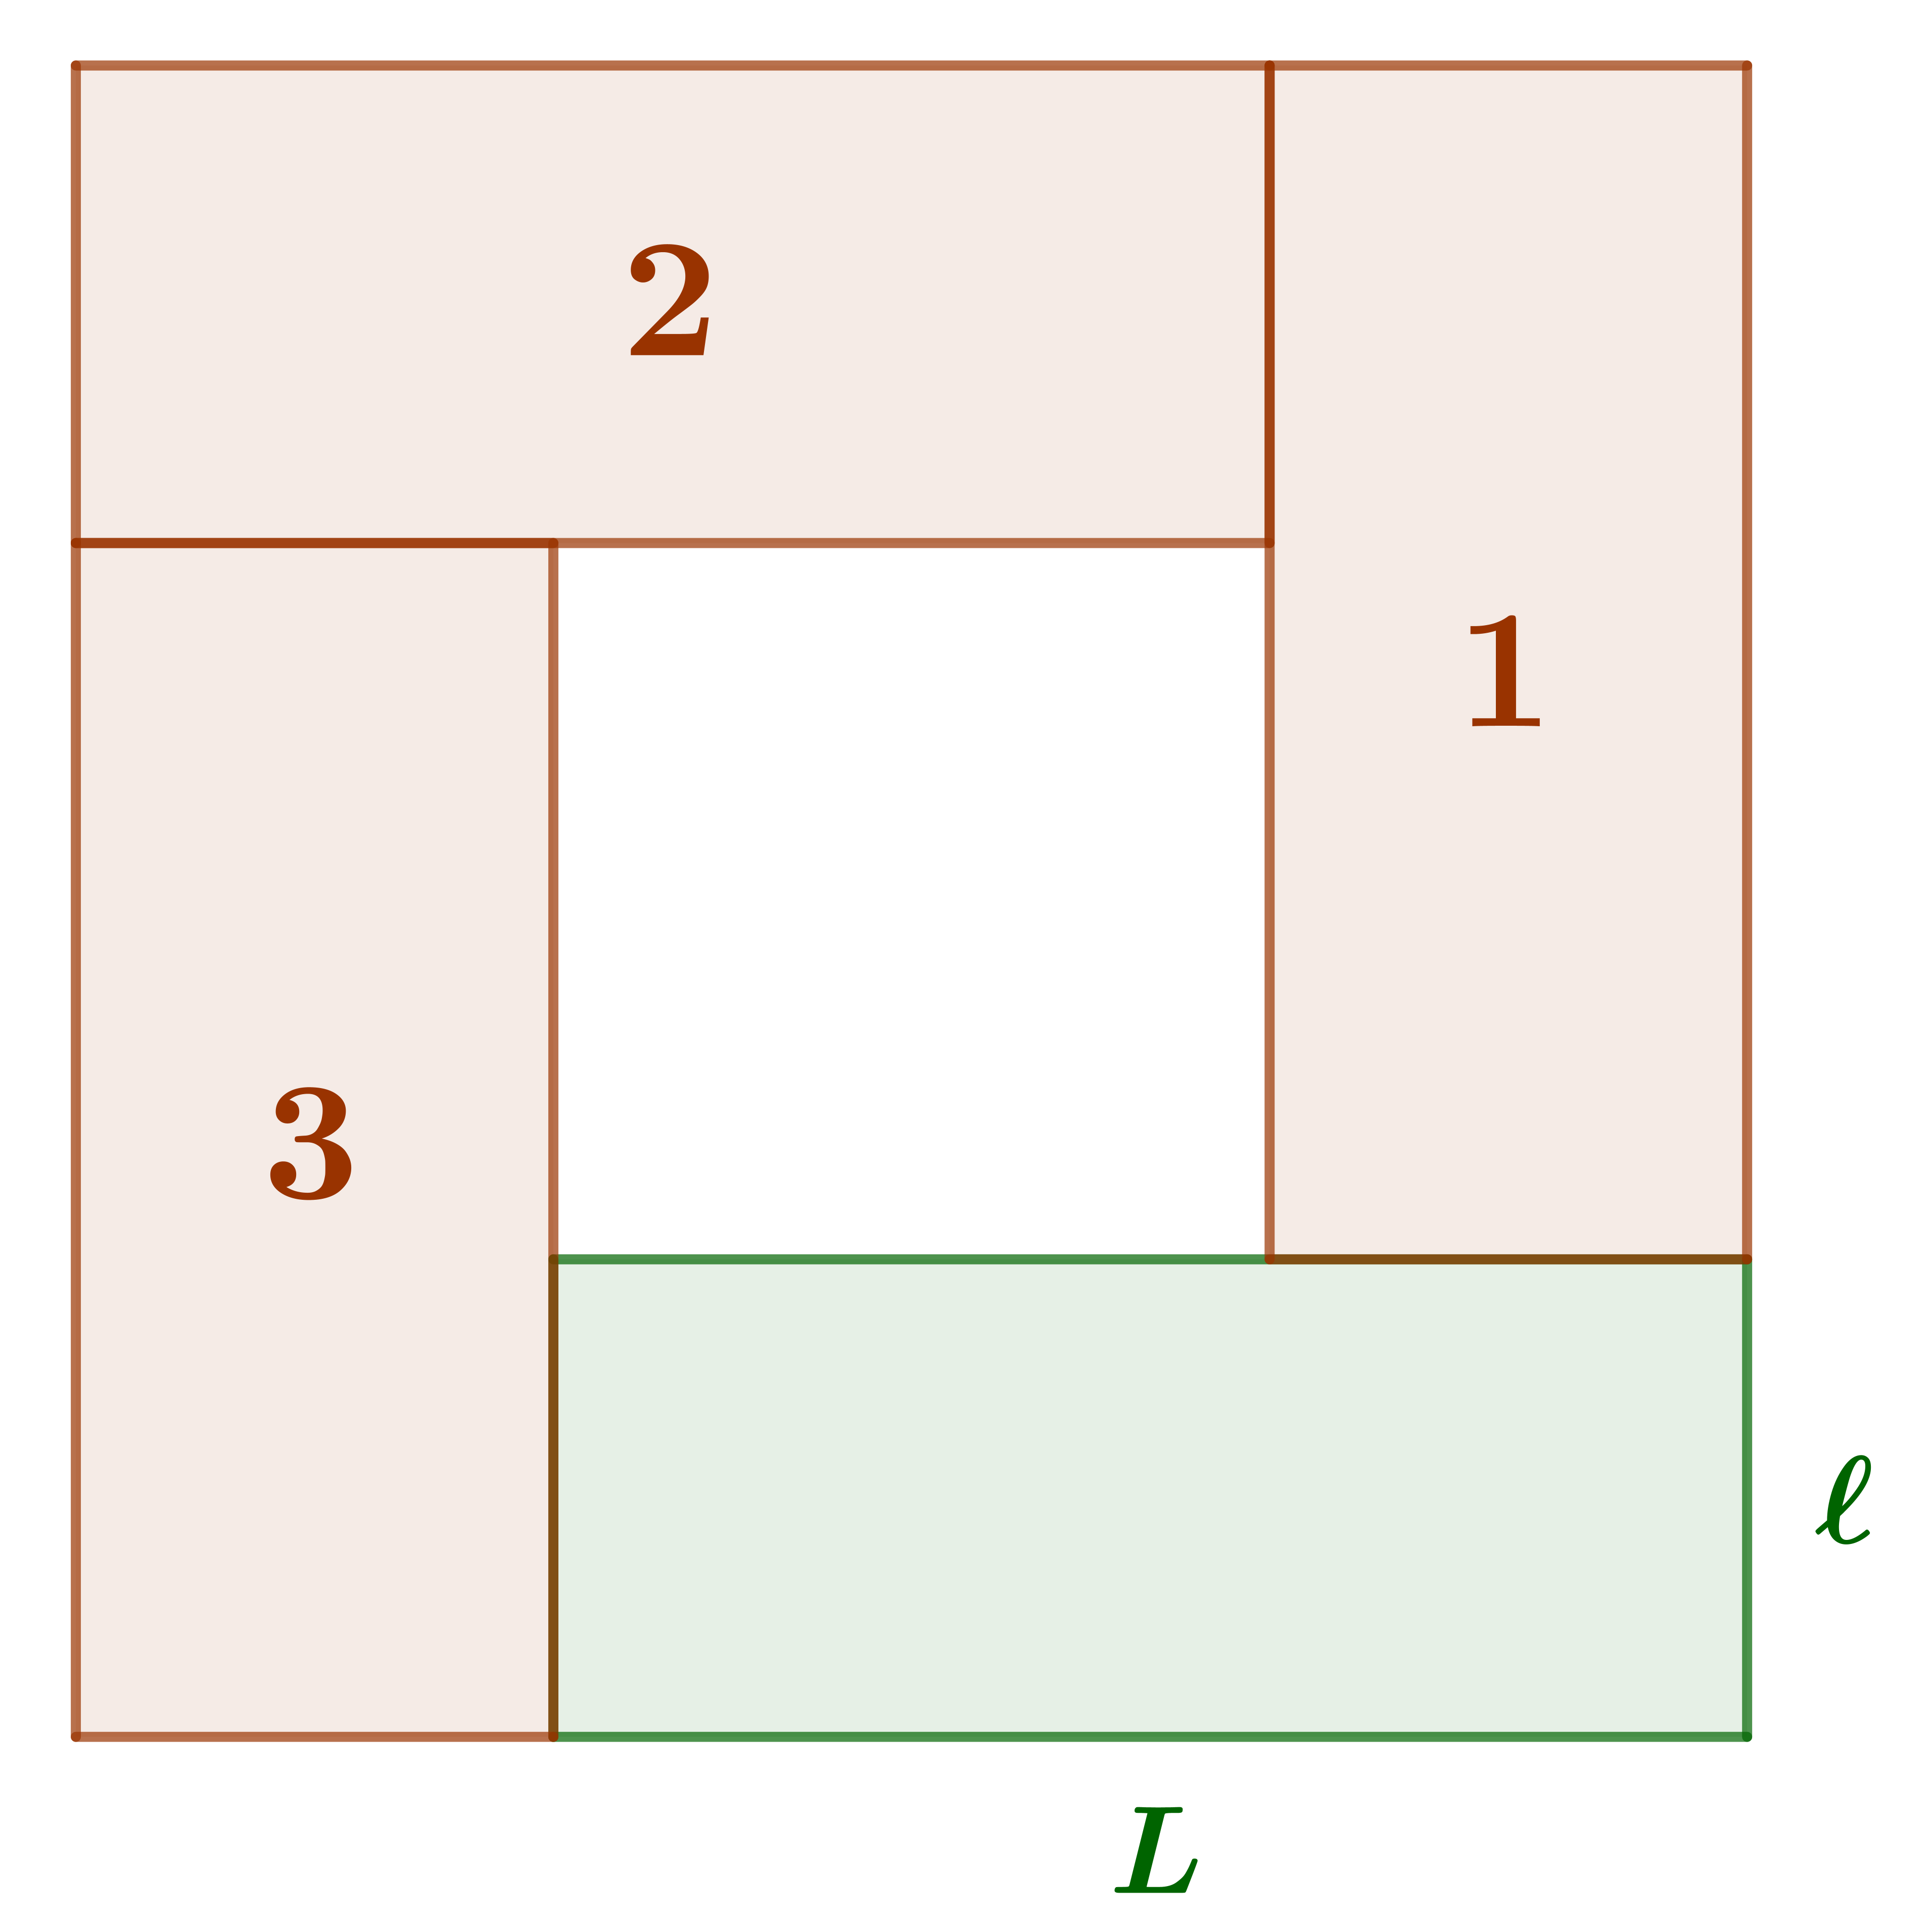
\includegraphics[scale=.4]{content/rectangle/rectangle.png}
	\end{center}
	
	Le raisonnement tient alors aux constations suivantes accessibles à un collégien.
	%
	\begin{enumerate}
		\item Le grand carré a une aire supérieure ou égale à $4 L \ell$.

		\item Le grand carré a un périmètre égal à $4 (L + \ell)$.

		\item Via une homothétie de rapport \num{.5}\,, nous obtenons un carré d'aire supérieure ou égale à $\num{.5}^2 \times 4 L \ell =  L \ell$, et de périmètre égal à $\num{.5} \times 4 (L + \ell) = 2 (L + \ell)$.
	\end{enumerate}
	
	Donc pour tout rectangle de périmètre $p = 2 (L + \ell)$ et d'aire $L \ell$, nous pouvons construire un carré de périmètre identique, mais avec une aire supérieure ou égale à  $L \ell$. Joli! Non?
\end{proof}


\begin{remark}
	Au passage, nous avons pour $(L ; \ell) \in \big( \RRsp \big)^2$, $4 L \ell \leq (L + \ell)^2$, c'est-à-dire $2 L \ell \leq L^2 + \ell^2$, d'où $\sqrt{L \ell} \leq \sqrt{\frac12 (L^2 + \ell^2)}$, soit la comparaison des moyennes géométriques et quadratiques d'ordre $2$.
\end{remark}



% ------------- %


\section{Le cas du parallélogramme}

\begin{fact} \label{iso-para}
	Considérons tous les parallélogrammes de périmètre fixé $p$. Parmi tous ces parallélogrammes, un seul est d'aire maximale, c'est le carré de côté $c = \num{.25} p$.
\end{fact}


\begin{proof}
	Le calcul de l'aire d'un parallélogramme, voir le dessin ci-dessous, nous donne 
	$\area{ABCD} = \area{ABHH^{\,\prime}}$ et 
	$\perim{ABCD} \geq \perim{ABHH^{\,\prime}}$, 
	avec égalité uniquement si $ABCD$ est un rectangle. 
	
	\begin{center}
		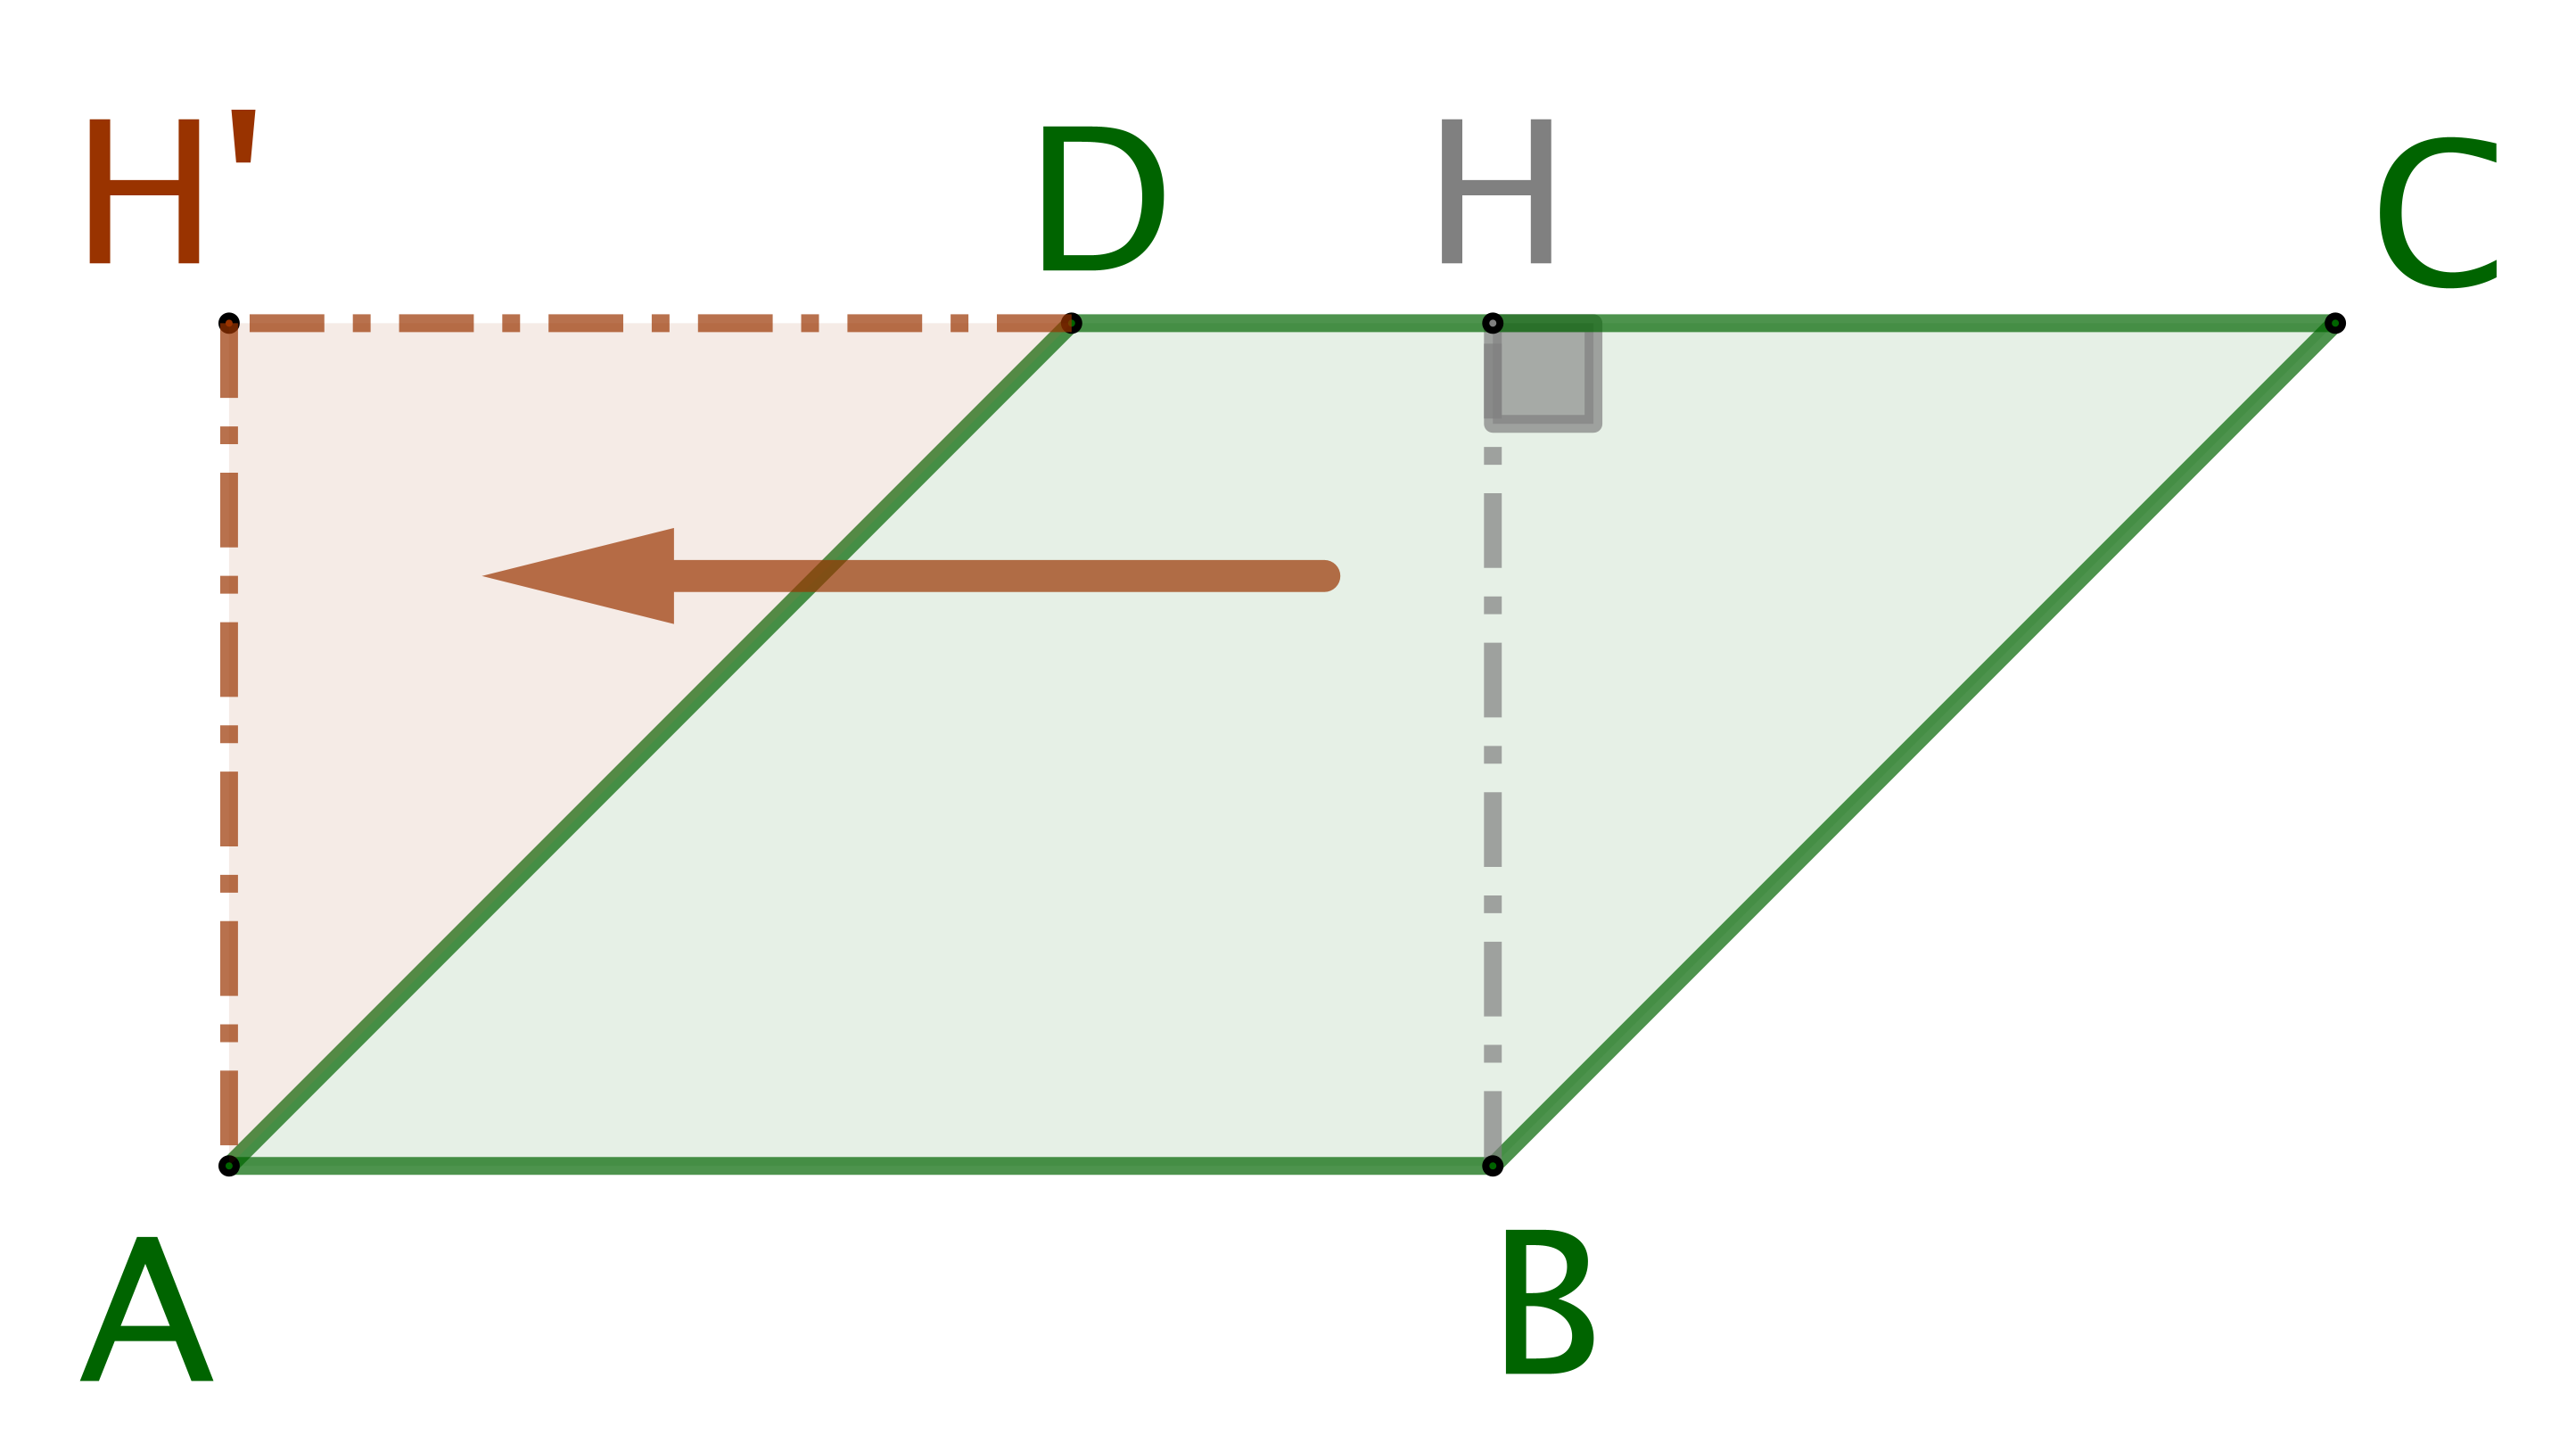
\includegraphics[scale=.4]{content/parallelogram/para-2-rect.png}
	\end{center}
	
	Via une homothétie de rapport $r = \frac{\perim{ABCD}}{\perim{ABHH^{\,\prime}}} \geq 1$, nous obtenons un rectangle 
	de périmètre égal à $p$,
	et d'aire supérieure ou égale à $\area{ABCD}$, 
	avec égalité uniquement si $ABCD$ est un rectangle.
	Nous revenons à la situation du fait \ref{iso-rect} qui permet de conclure très facilement.
\end{proof}


% ----------------------- %


\begin{remark}
	Une méthode analytique devient pénible ici, car il faut, par exemple, prendre en compte l'angle au sommet $A$ du parallélogramme. L'auteur préfère battre en retraite en clôturant cette remarque ici.
%	\footnote{
%		Et oui, l'auteur est un lâche.
%	}
\end{remark}



% ------------- %


\section{Le cas du triangle}

\begin{fact}\label{iso-tri}
	Considérons tous les triangles de périmètre fixé $p$. Parmi tous ces triangles, celui d'aire maximale est le triangle équilatéral de côté $c = \dfrac13 p$.
\end{fact}


\begin{proof}
	Une première idée, calculatoire, est de passer via la classique formule de Héron $Aire = \sqrt{s(s - a)(s - b)(s - c)}$ où $s = \num{.5} p$ désigne le demi-périmètre, et les variables $a$, $b$ et $c$ les mesures des côtés du triangle. Concrètement, comme l'aire est positive ou nulle, il suffit de chercher les minimums de $Aire^2 = s(s - a)(s - b)(s - c)$. Ceci fonctionne, mais n'est pas accessible à un collégien, ni même à un lycéen qui ne sait pas différentier une fonction de plusieurs variables.%
	\footnote{
		XXXX
		
		L'ensemble des valeurs possibles de $a$, $b$ et $c$ est un compact, quitte à accepter des triangles dégénérés, donc  atteint son minimum.
		Comme de plus, les antécédents de ce minimum doivent annuler $\pder{A_s}{a}{1}$, $\pder{A_s}{b}{1}$ et $\pder{A_s}{c}{1}$, et $A_s(a;b;c)$ est une fonction symétrique en $a$, $b$ et $c$, nous savons que le minimum est atteint en $(\frac13 p ; \frac13 p ; \frac13 p)$. 
	}
	Il se trouve que l'on peut établir l'affirmation \ref{iso-tri} ci-dessus avec des raisonnements géométriques élémentaires.
	La petite astuce toute simple est de considérer le problème plus contraint exprimé dans le fait \ref{iso-tri-one-side-fixed} ci-dessous qui permet de conclure comme suit.
	%
	\begin{itemize}
		\item 

		\item 

		\item 
	\end{itemize}
\end{proof}


% ----------------------- %


\begin{fact}\label{iso-tri-one-side-fixed}
	Considérons tous les triangles de périmètre fixé $p$ et ayant tous au moins un côté de même mesure $c$. Parmi tous ces triangles, celui qui a une aire maximale est le triangle isocèle ayant une base de mesure $c$.
\end{fact}


\begin{proof}
	XXXX

	\begin{center}
		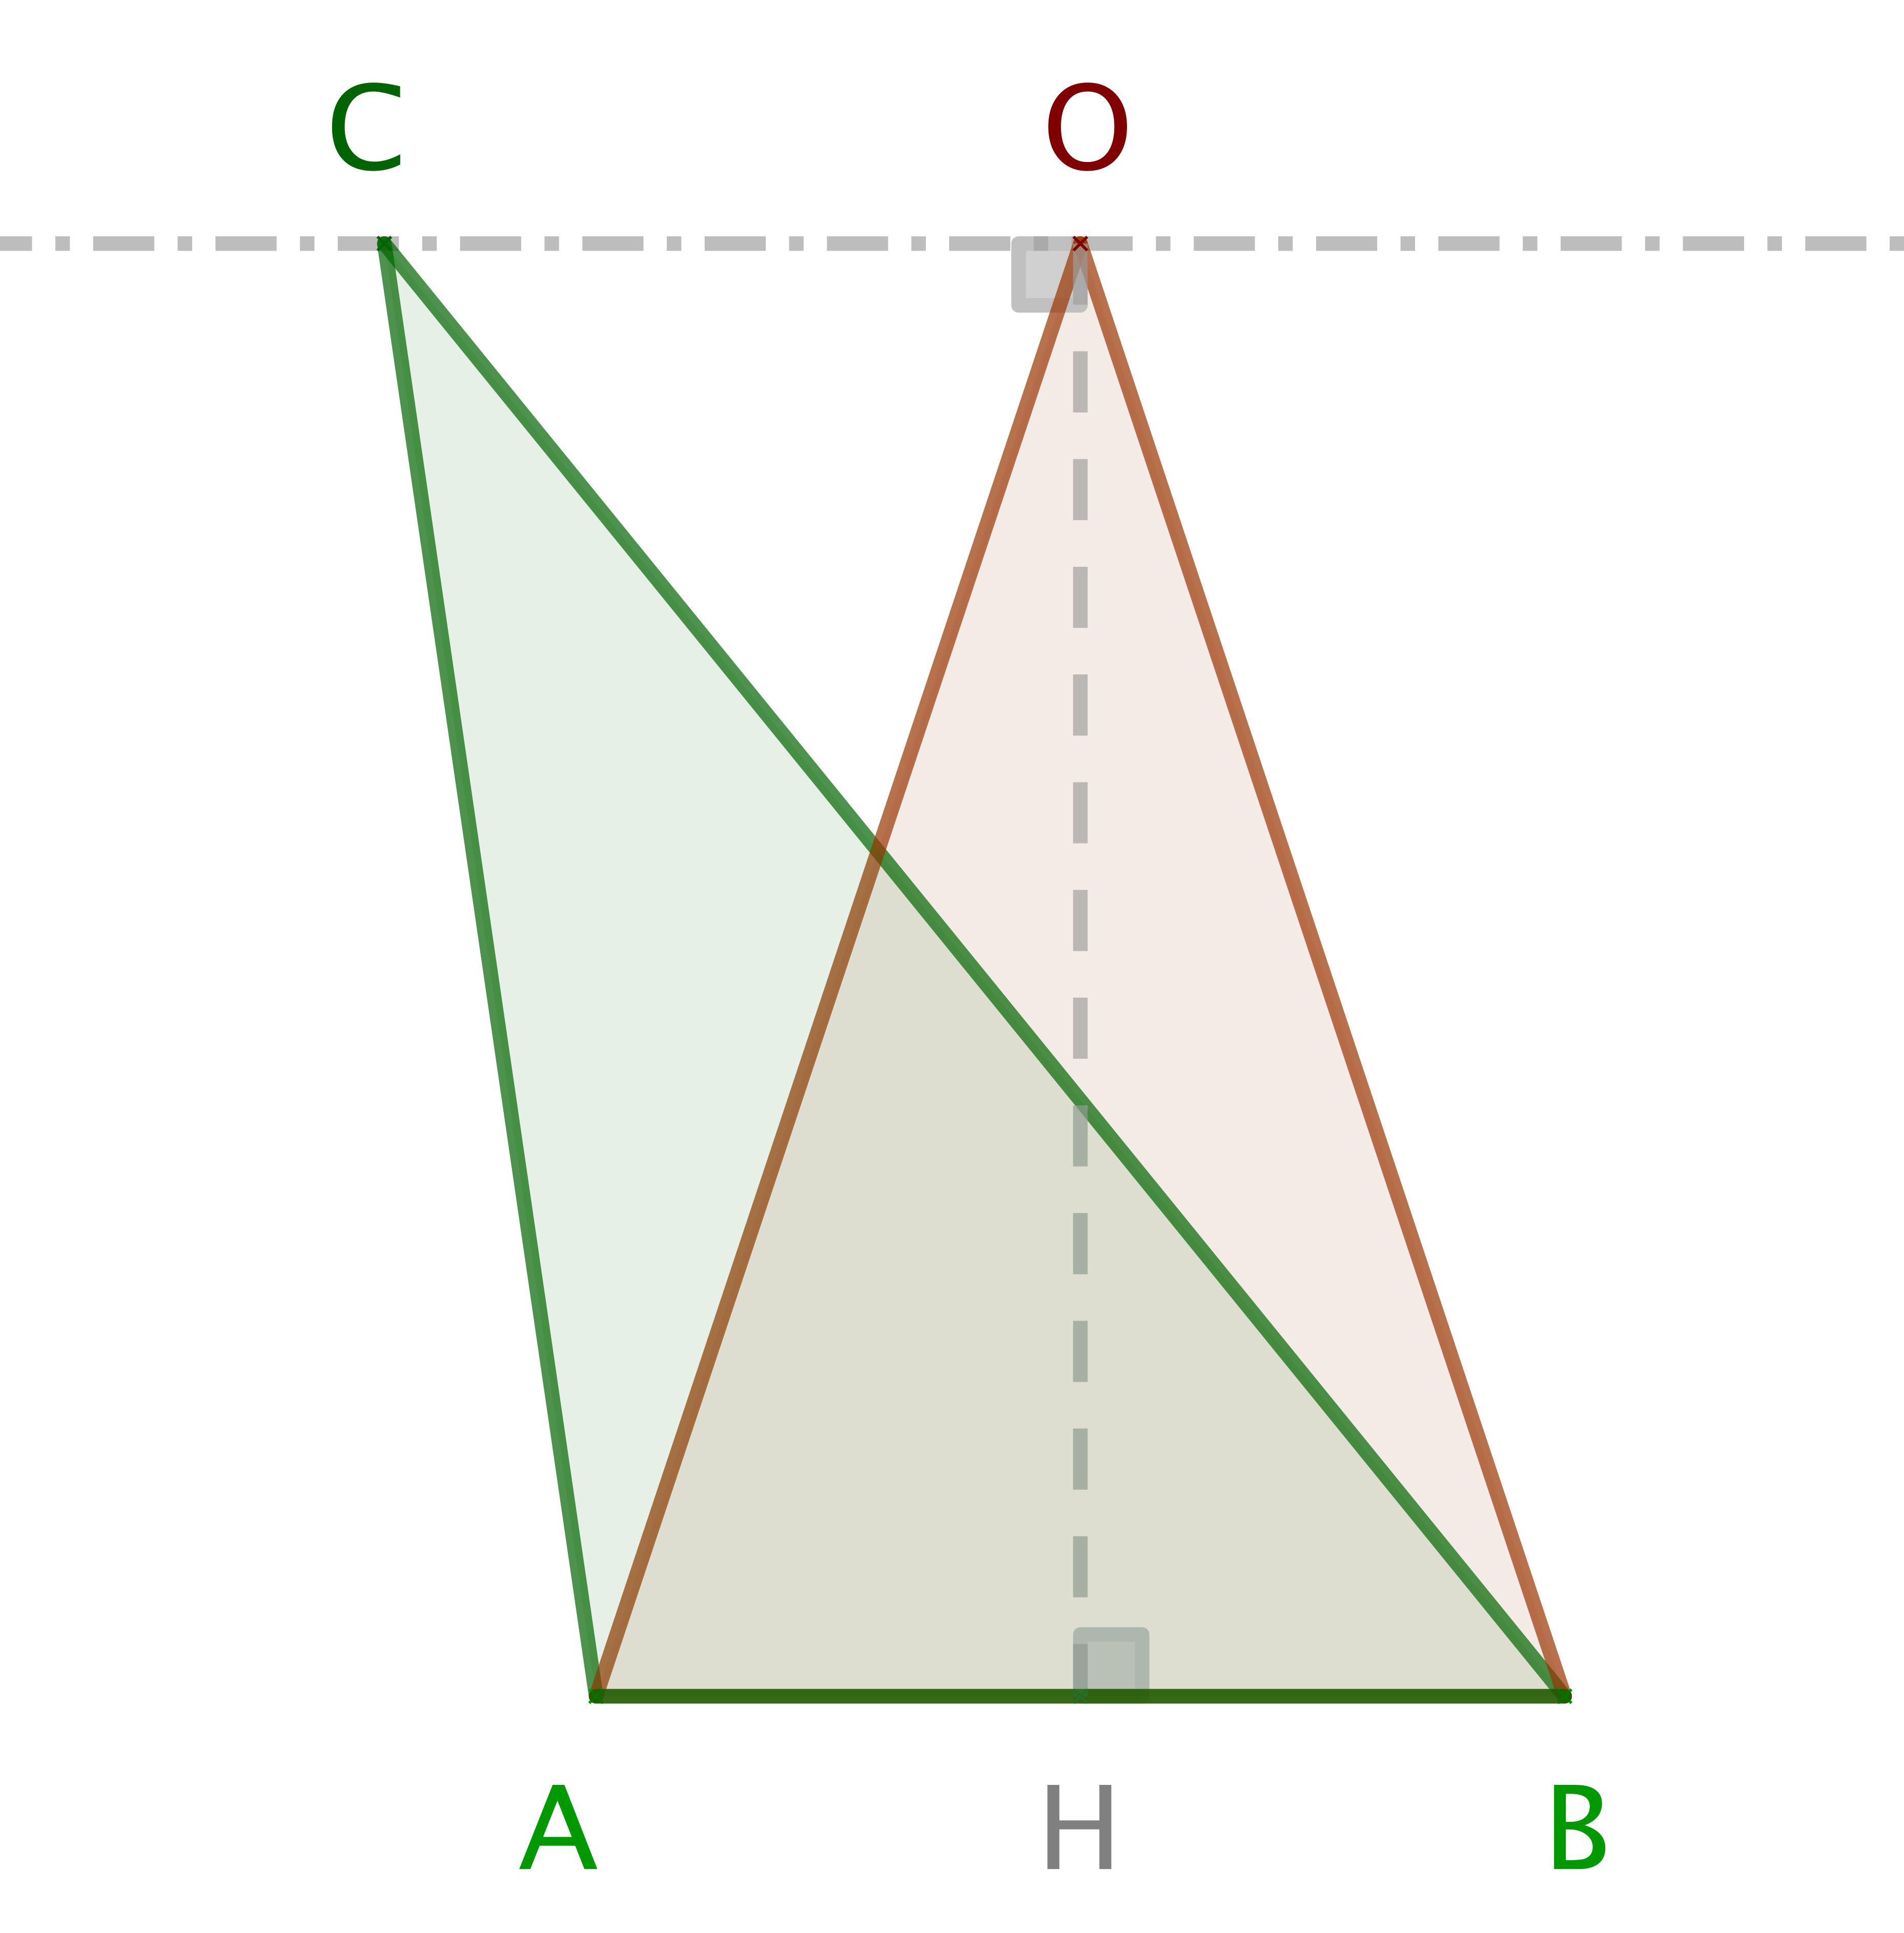
\includegraphics[scale=.4]{content/triangle/triangle.png}
	\end{center}

	\begin{center}
		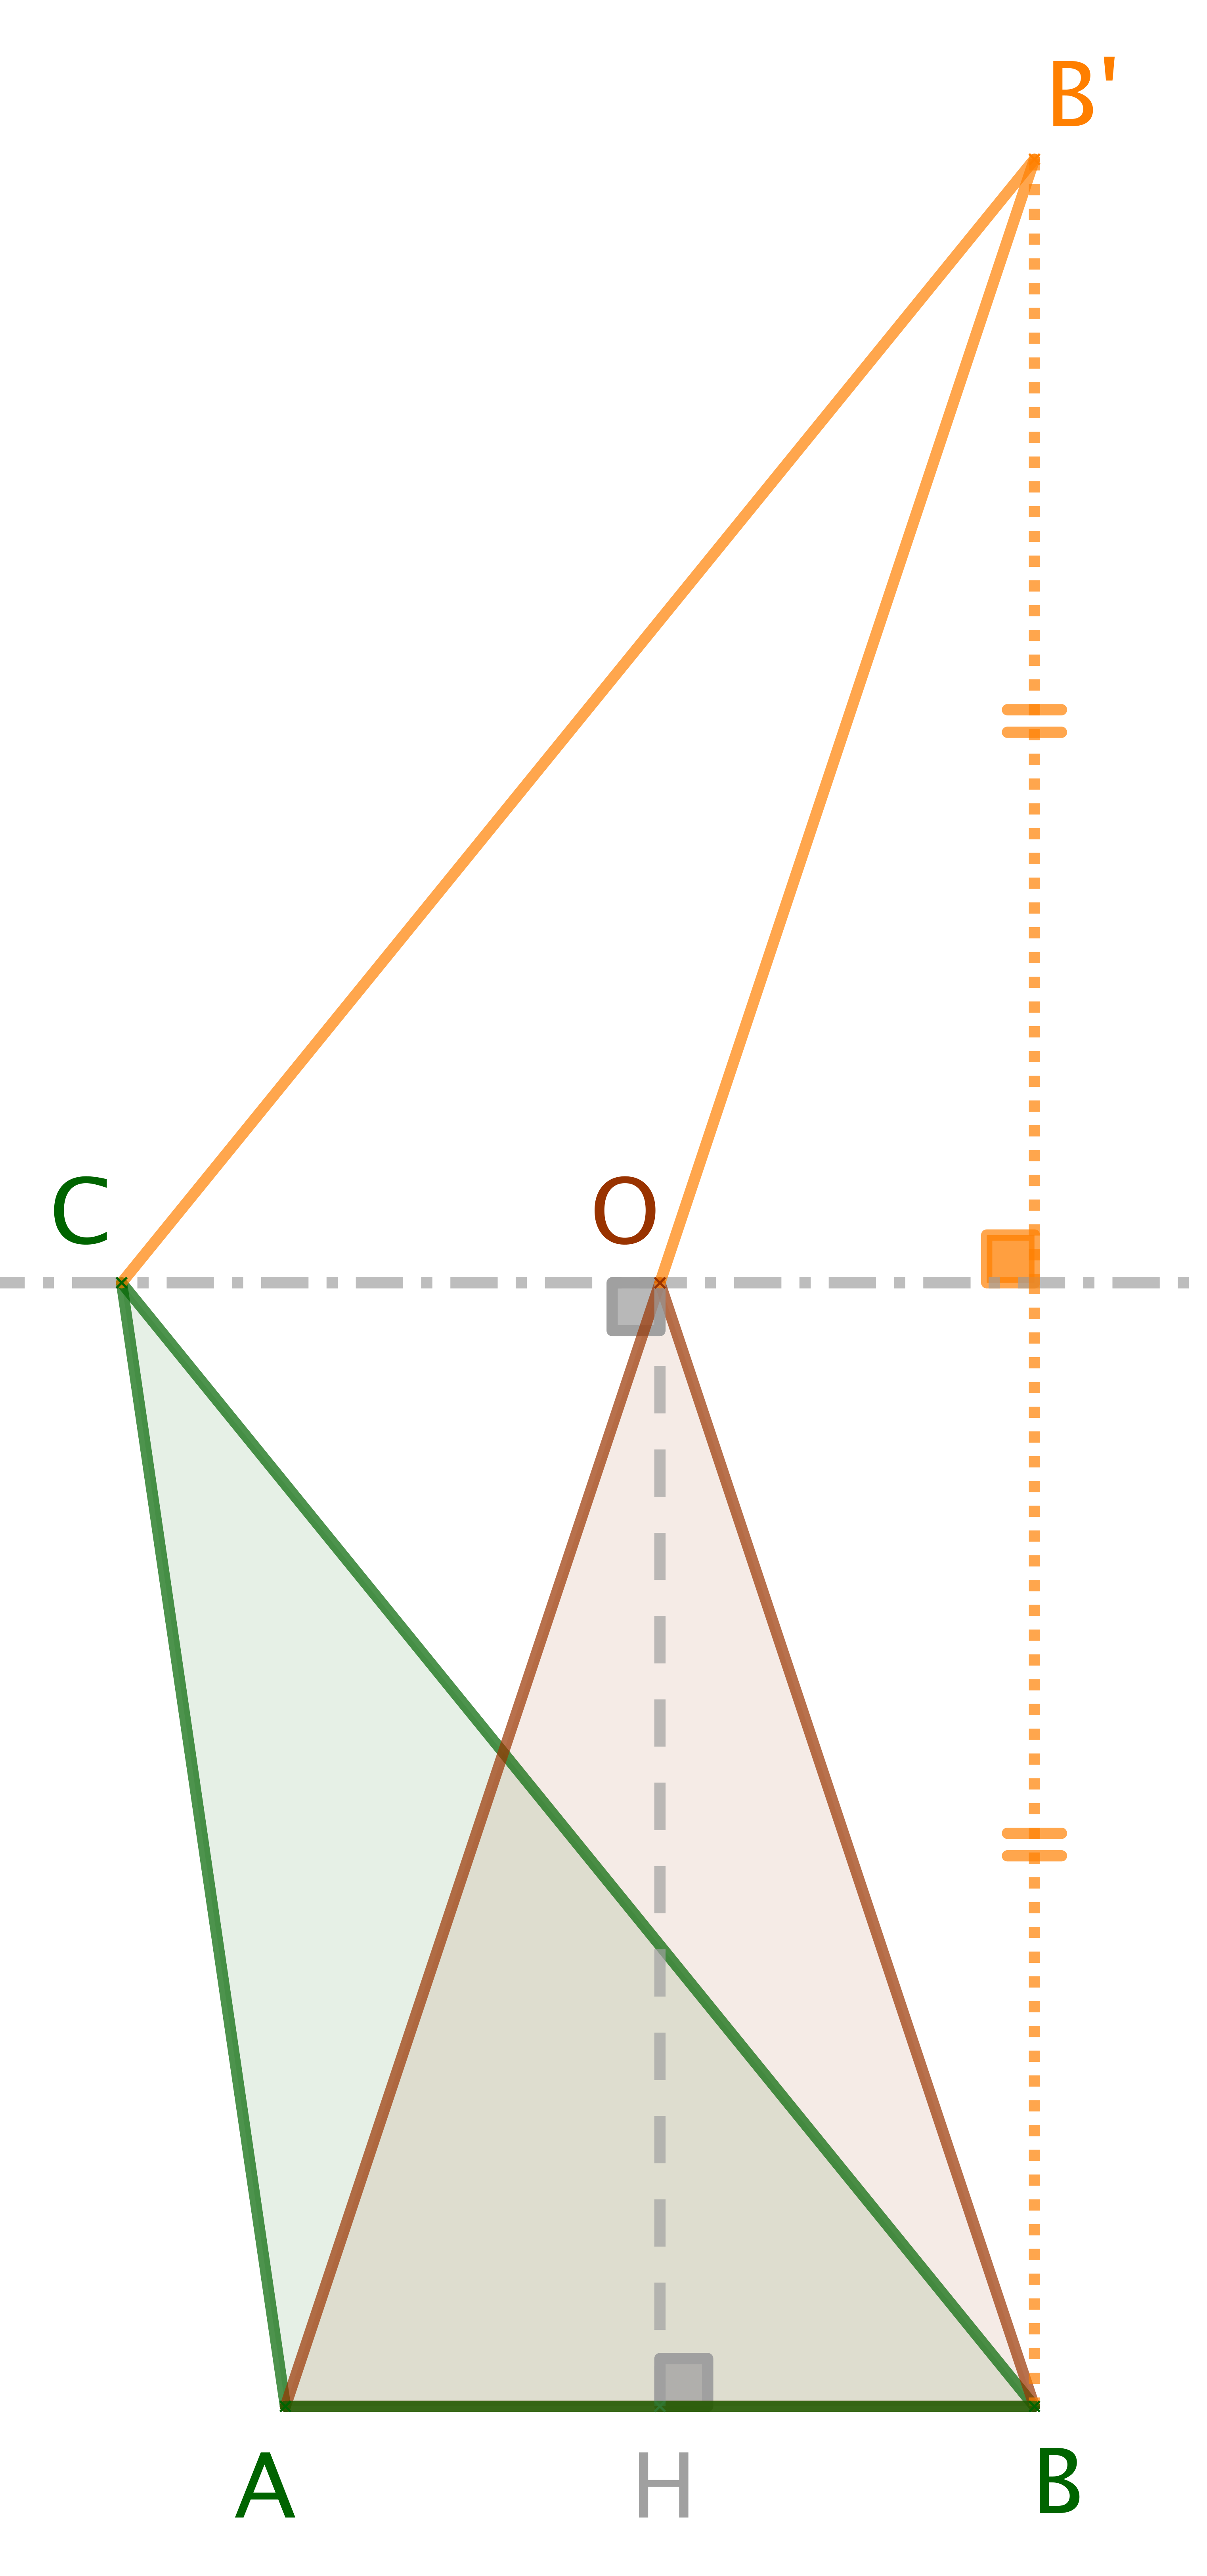
\includegraphics[scale=.4]{content/triangle/triangle-proof.png}
	\end{center}
	
	YYYY
	
	
	Joli! Non?
\end{proof}


% ------------- %


%\section{Le cas du quadrilatère}
%
%\begin{fact}
	Considérons tous les quadrilatères de périmètre fixé $p$. Parmi tous ces quadrilatères, celui d'aire maximale est le carré de côté $c = \num{.25} p$.
\end{fact}


\begin{proof}
	La figure suivante montre que pour tout quadrilatère $ABCD$ non convexe en $B$, et de périmètre $p$, il existe un quadrilatère convexe $AB^{\,\prime}CD$ de périmètre $p$, et tel que $\area{AB^{\,\prime}CD} \geq \area{ABCD}$.
	Notre recherche doit donc continuer dans l'ensemble des quadrilatères convexes de périmètre $p$.

	\begin{center}
		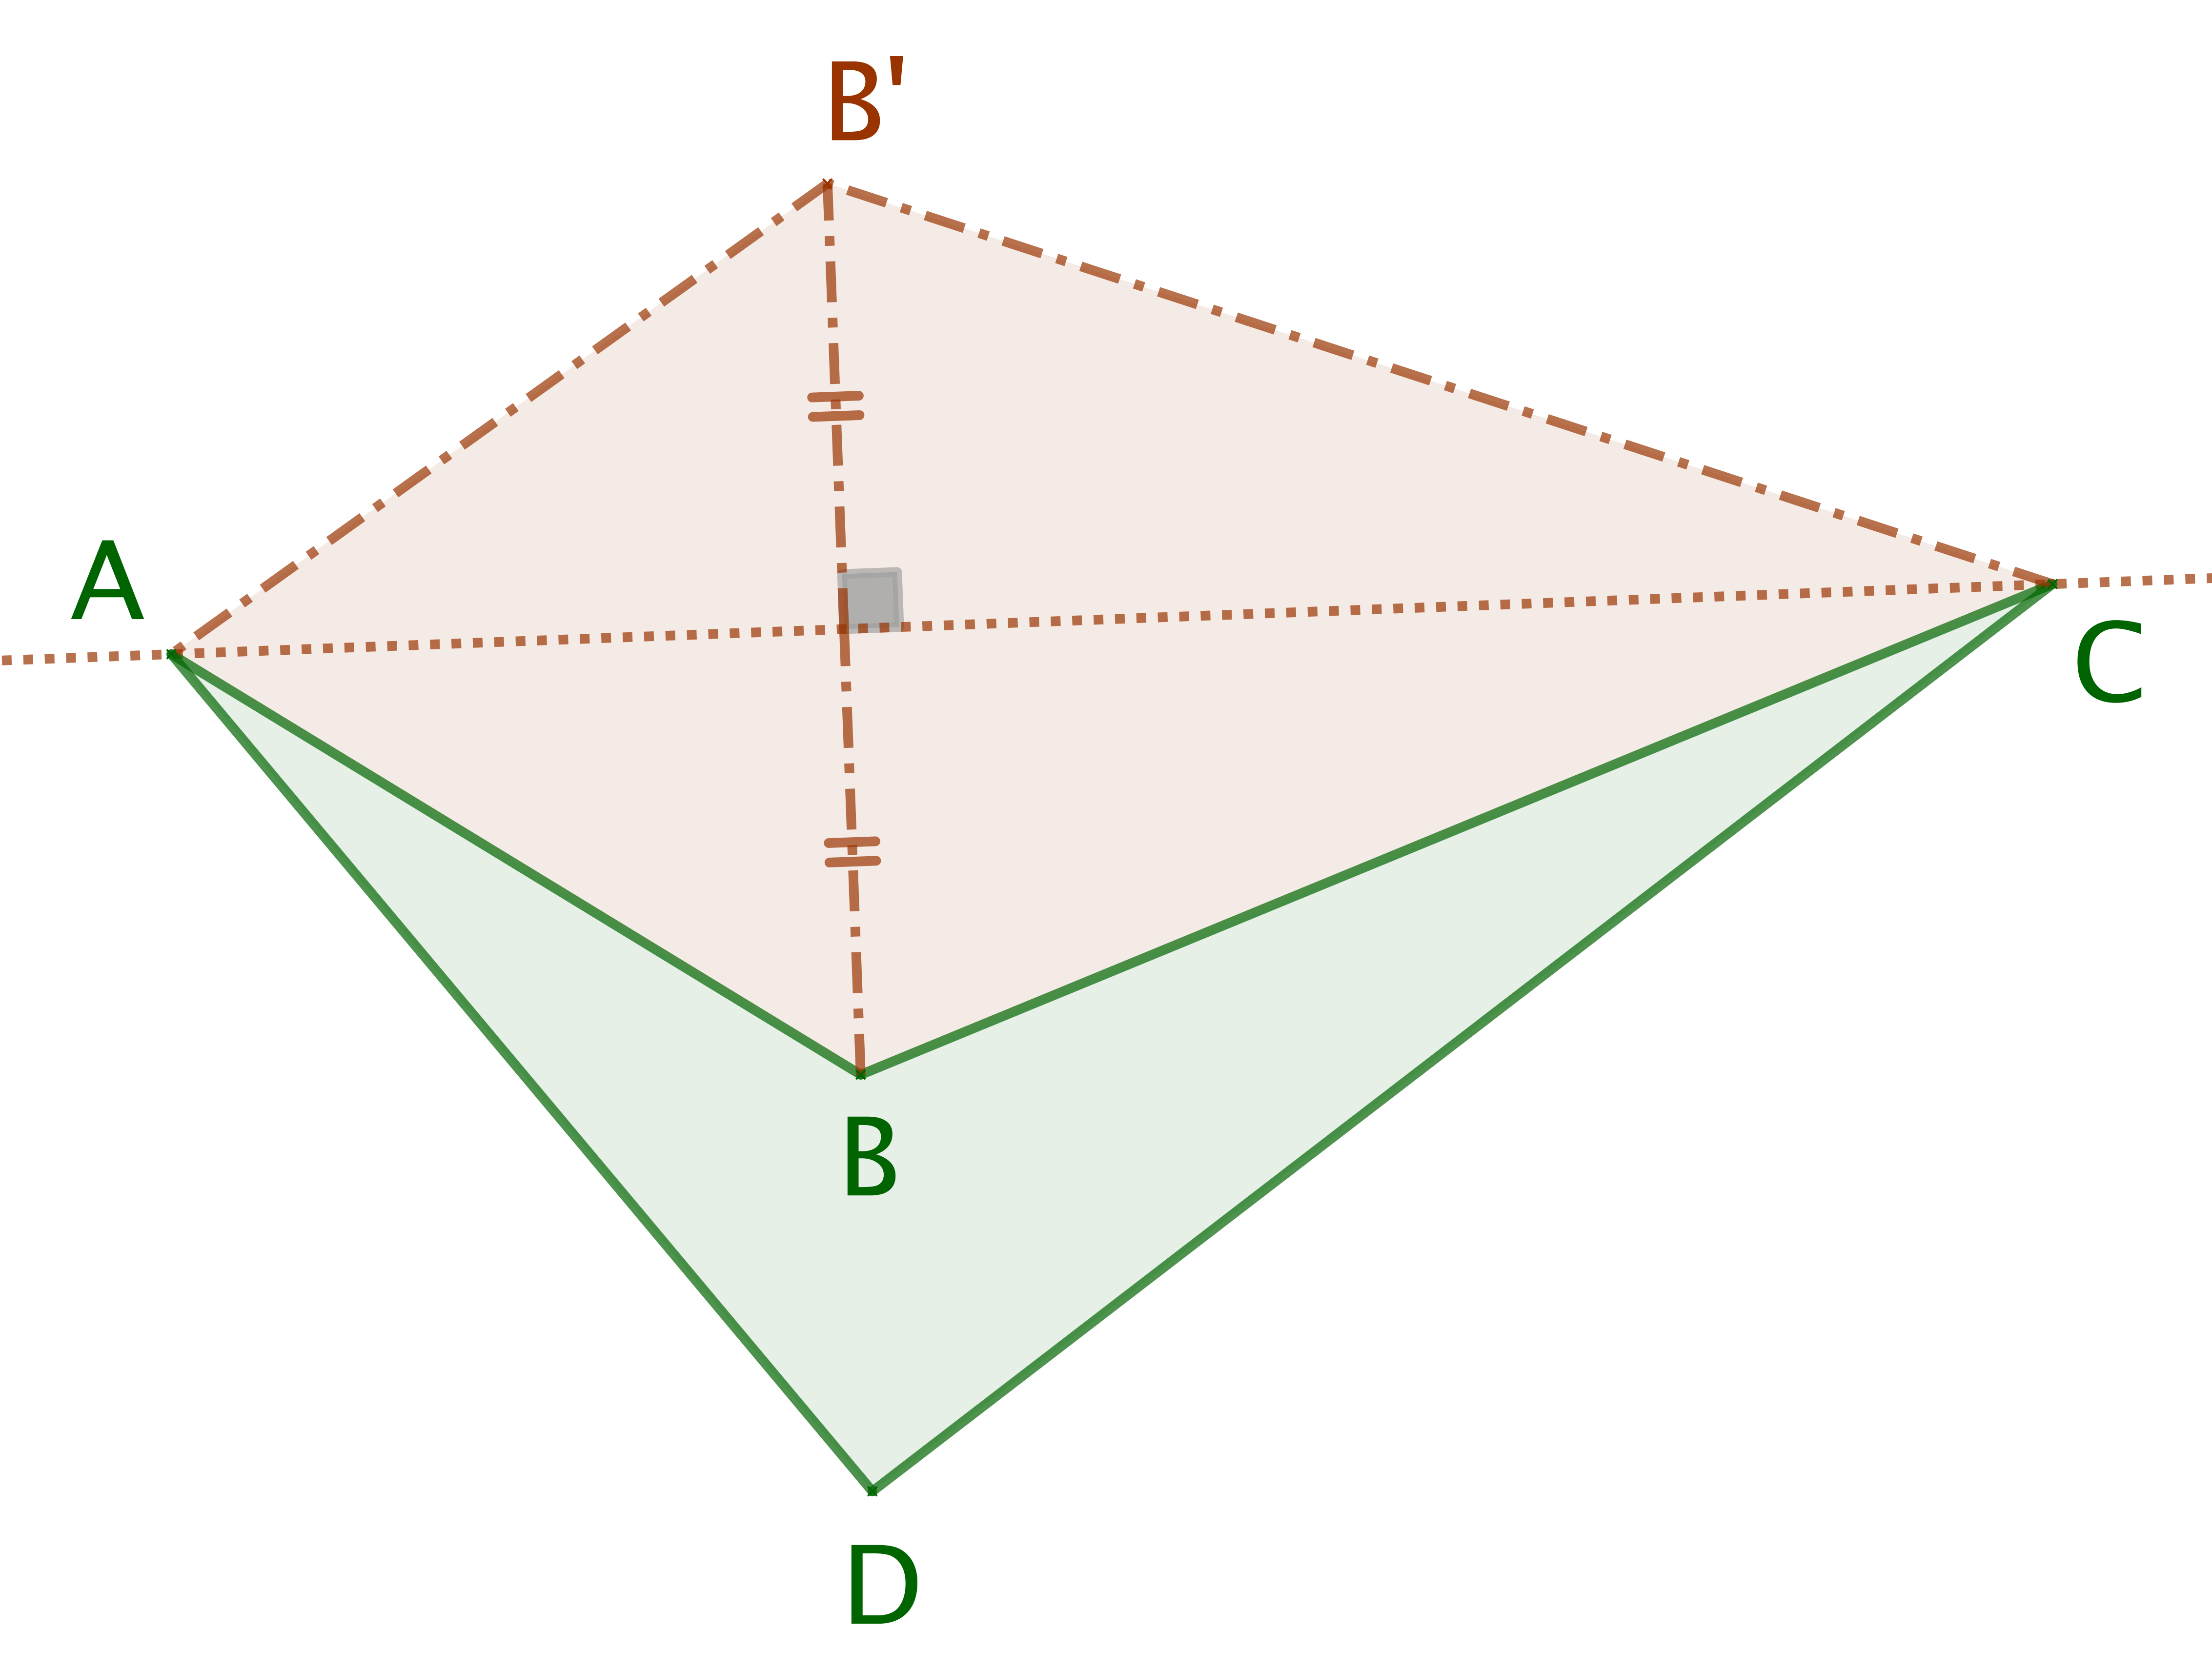
\includegraphics[scale=.4]{content/quadrilateral/quadrilateral-non-convex.png}
	\end{center}
	
	
	Comme dans la preuve du fait \ref{iso-tri-one-side-fixed}, à partir d'un quadrilatère convexe $ABCD$ de périmètre $p$, nous obtenons un quadrilatère convexe $AB^{\,\prime}CD$ de périmètre $p$,%
	\footnote{
		Noter que
		$\perim{AB^{\,\prime}CD} = \perim{AB^{\,\prime}C} + \perim{ACD} - 2 AC$.
	}
	et tel que $AB^{\,\prime} = B^{\,\prime}C$ et $\area{AB^{\,\prime}CD} \geq \area{ABCD}$ comme le montre la figure ci-après. 

	\begin{center}
		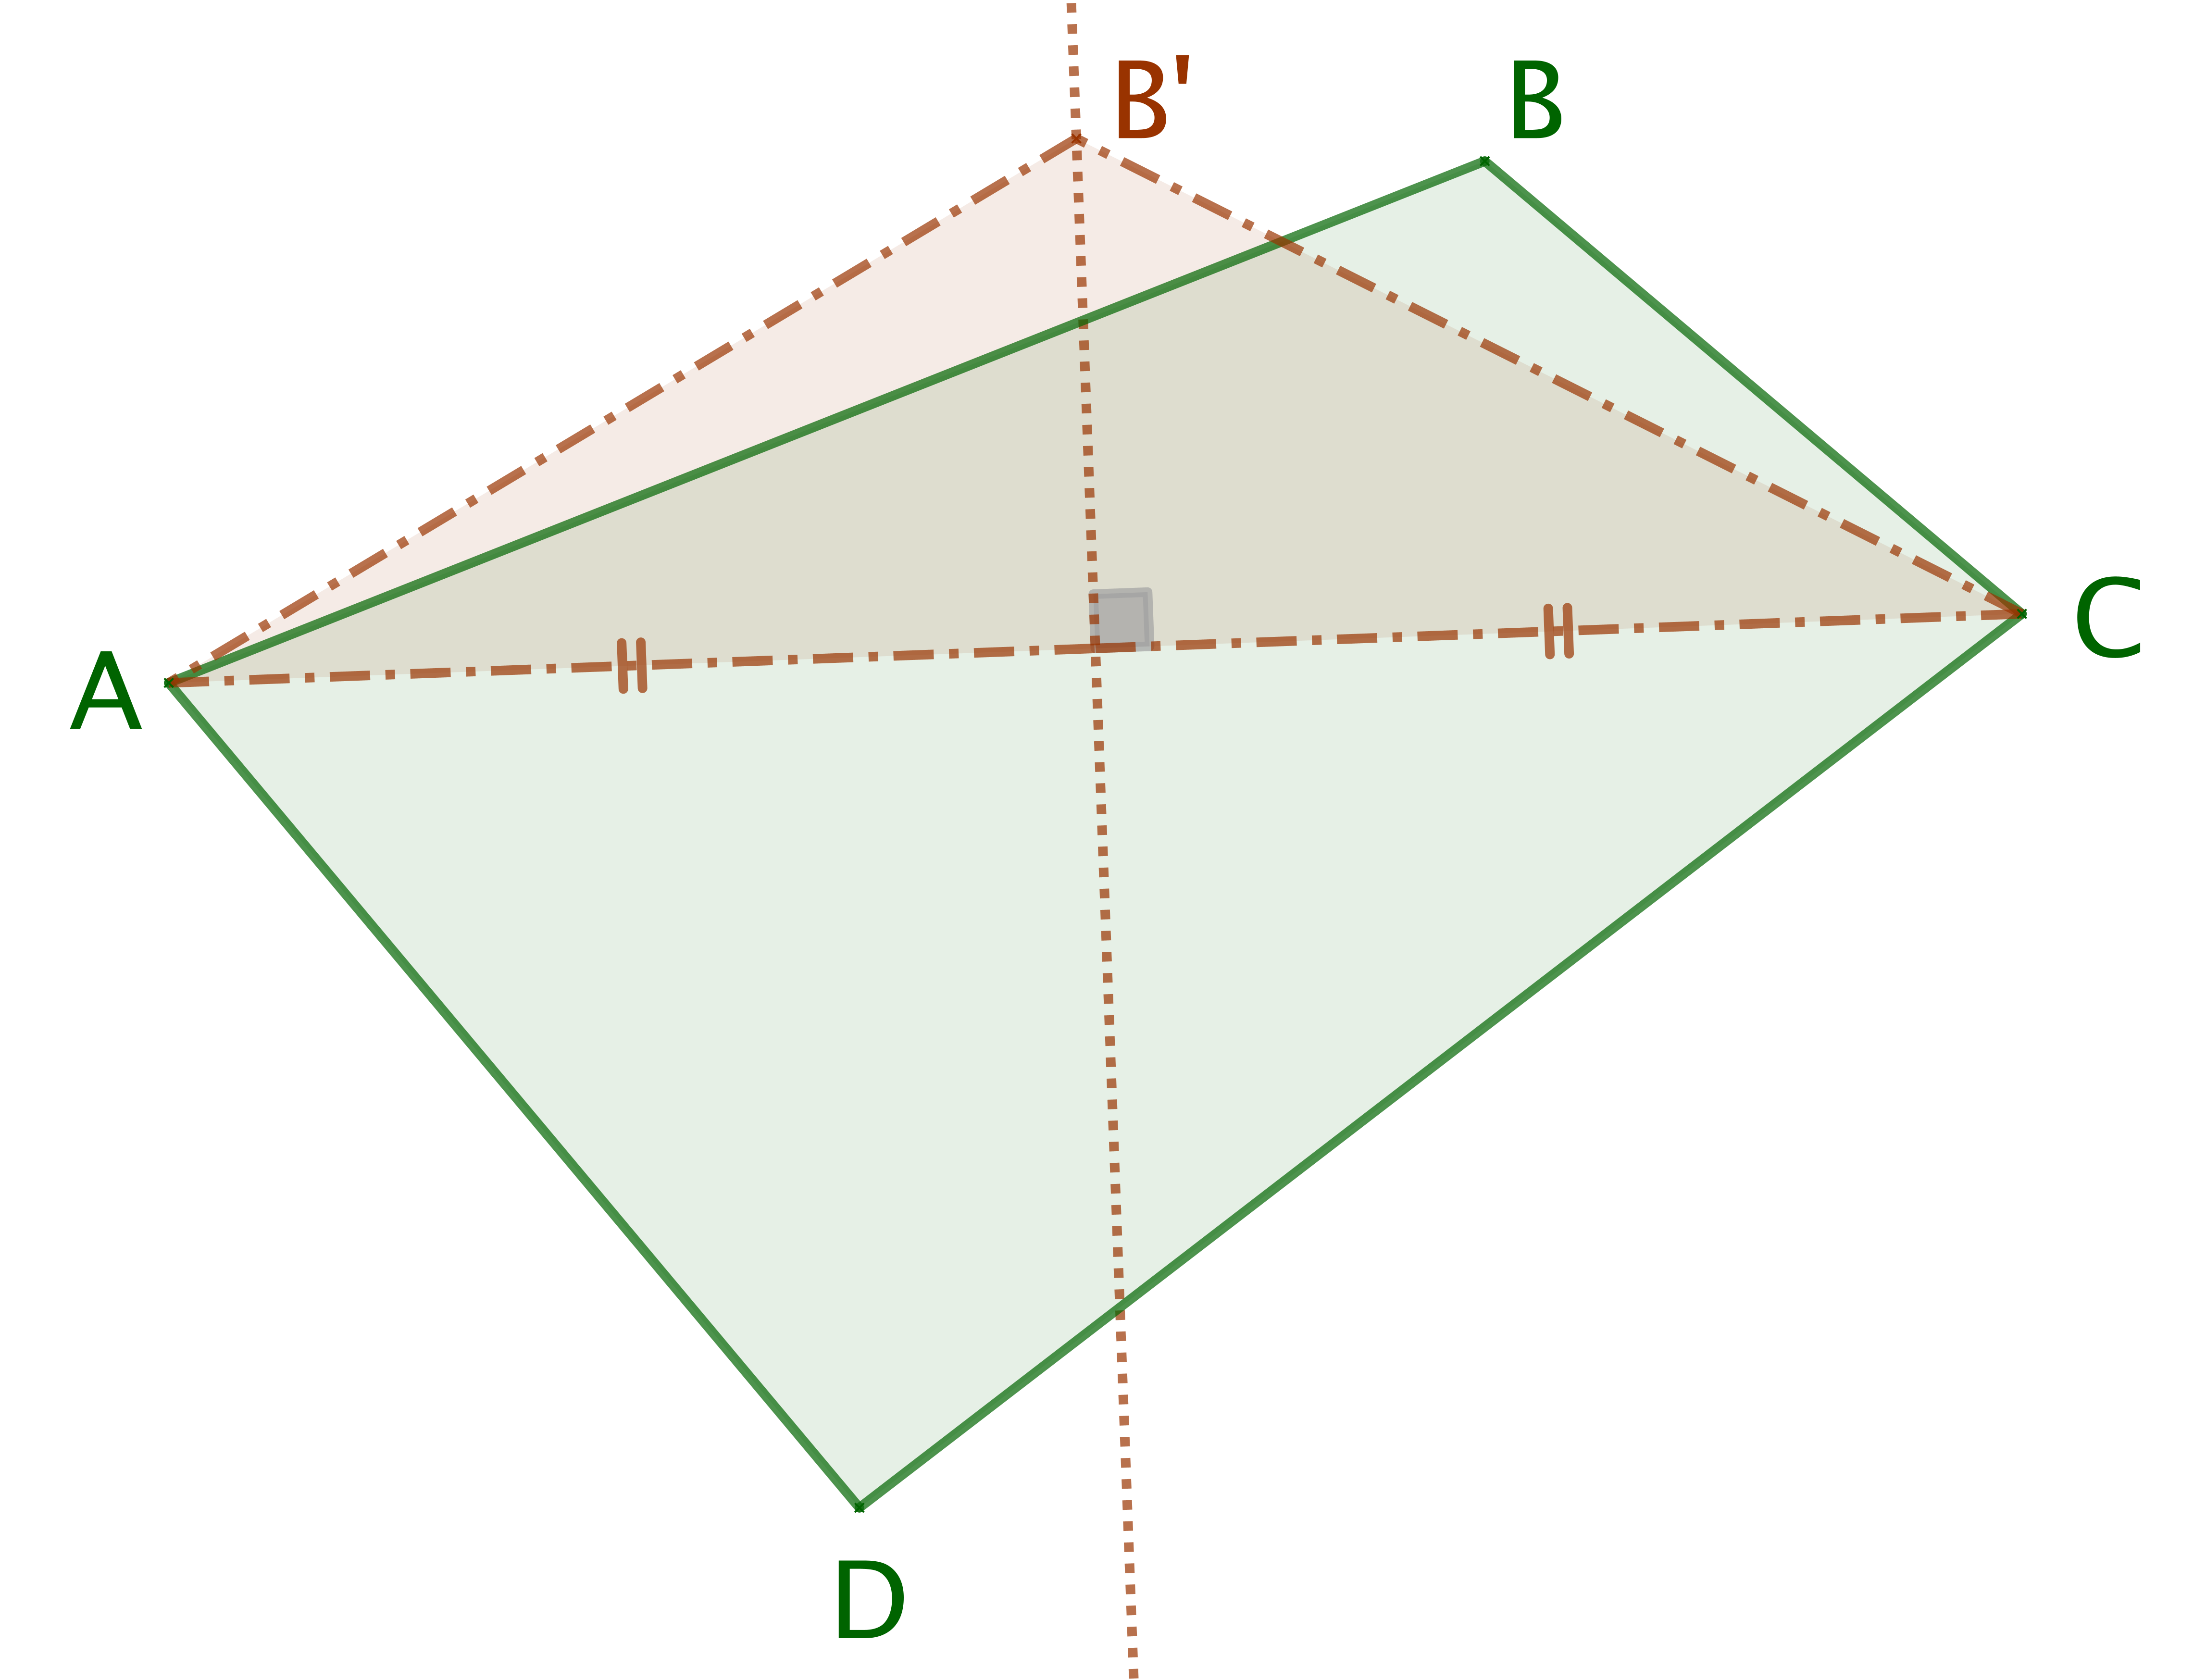
\includegraphics[scale=.4]{content/quadrilateral/quadrilateral-convex-gene.png}
	\end{center}
	
	
	La méthode précédente appliquée au sommet $D$ donne un cerf-volant $ABCD$ de périmètre $p$, et tel que $AB = BC$ et $AD = DC$, voir ci-dessous. 
	Cette même méthode avec les sommets $A$ et $C$ fournit un losange $A^{\,\prime}BC^{\,\prime}D$ de périmètre $p$, et tel que $\area{A^{\,\prime}BC^{\,\prime}D} \geq \area{ABCD}$.
	%
	En effet, nous avons
	$p = 2(AB + AD)$
	et
	$\perim{A^{\,\prime}BD} = \perim{ABD}$,
	donc
	$A^{\,\prime}B = A^{\,\prime}D = \num{.25} p$,
	et de même, nous obtenons
	$C^{\,\prime}B = C^{\,\prime}D = \num{.25} p$.

	\begin{center}
		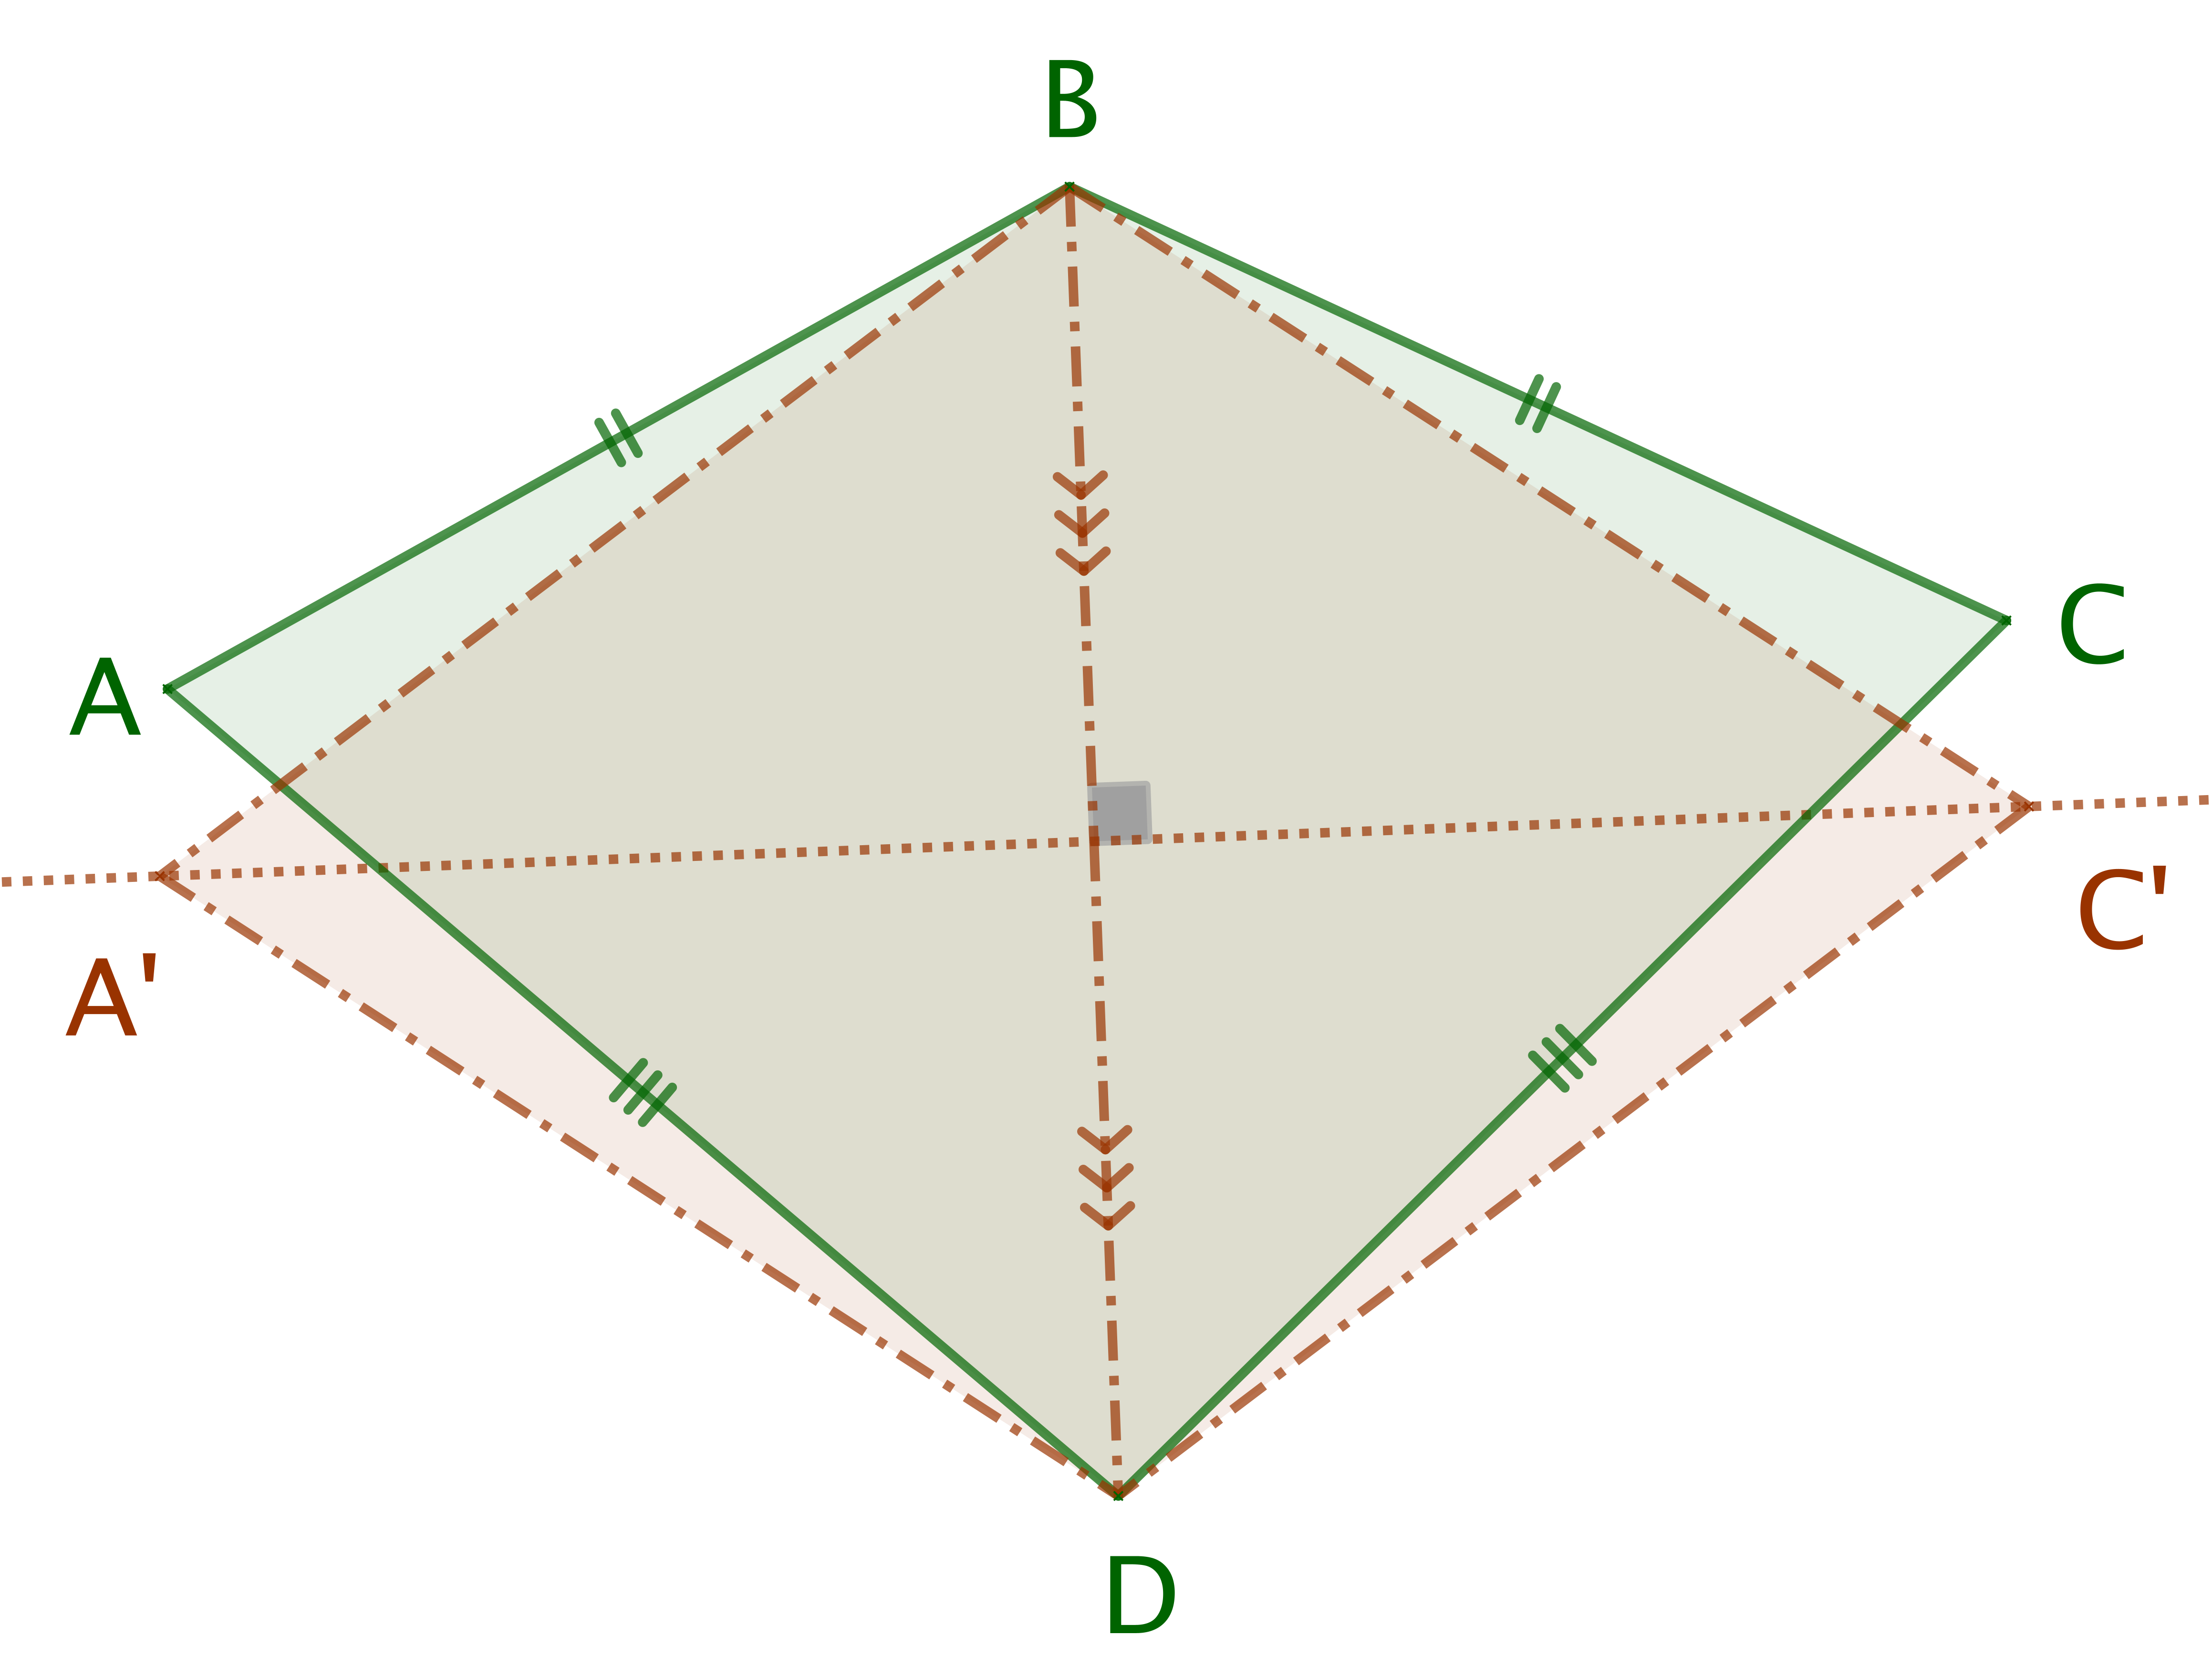
\includegraphics[scale=.4]{content/quadrilateral/quadrilateral-convex-isopaire.png}
	\end{center}
	
	
	Pour conclure, il suffit d'appliquer le fait \ref{iso-para}, puisque tout losange est un parallélogramme. Que la géométrie est belle!
\end{proof}



\end{document}
